\documentclass[border=2pt]{standalone}
\usepackage{verbatim}
\usepackage{tikz}
\begin{document}
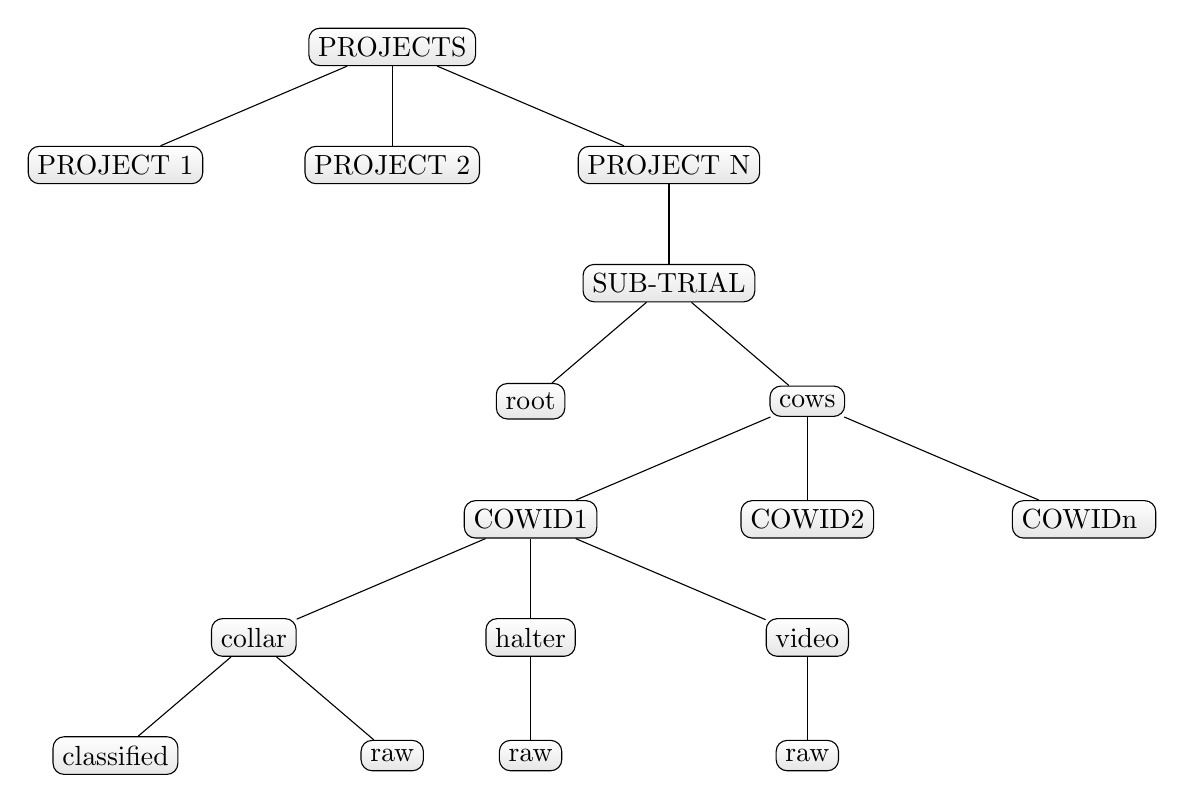
\begin{tikzpicture}[sibling distance=10em,
  every node/.style = {shape=rectangle, rounded corners,
    draw, align=center, top color=white, bottom color=black!10}]]
  \node {PROJECTS}
    child { node{PROJECT 1} }
    child { node{PROJECT 2} }
    child { node{PROJECT N}
        child { node {SUB-TRIAL}
            child { node {root} }
            child { node {cows}
                child { node {COWID1}
                    child { node {collar}
                        child { node {classified} }
                        child { node {raw} }
                    }
                    child { node {halter}
                        child { node {raw} }
                    }
                    child { node {video}
                        child { node {raw} }
                    }
                }
                child { node {COWID2} }
                child { node {COWIDn } }
            }
        }
    };

\end{tikzpicture}
\end{document}
